
As in \cite{schm11}, the computational domain is $1000km \times 660km$.
No-slip boundary conditions are imposed on the sides of the system while free-slip
boundary conditions are imposed at the top and bottom.
Two materials are present in the domain: the lithosphere (mat.1) and the mantle (mat.2). 
The overriding plate (mat.1) is $80km$ thick and is placed at the top of the domain. 
An already subducted slab (mat.1) of $250km$ length hangs vertically under this plate.
The mantle occupies the rest of the domain.

The mantle has a constant viscosity $\eta_0=10^{21}Pa.s$ and a density $\rho=3150kg/m^3$. 
The slab has a density $\rho=3300kg/m^3$ and is characterised by a power-law flow law so that 
its effective viscosity depends on the second invariant of the strainrate $I_2$ as follows:

\begin{equation}
\eta_{eff}
=\frac{1}{2} A^{-1/n_s} I_2^{1/n_s-1} 
=\frac{1}{2} [(2 \times 4.75\!\times\! 10^{11})^{-n_s}]^{-1/n_s} I_2^{1/n_s-1} 
=4.75\!\times\! 10^{11} I_2^{1/n_s-1} 
= \eta_0 I_2^{1/n_s-1} 
\end{equation}
with 
$n_s=4$ and $A=(2 \times 4.75\!\times\! 10^{11})^{-n_s}$, or $\eta_0=4.75\times 10^{11}$.




\begin{center}
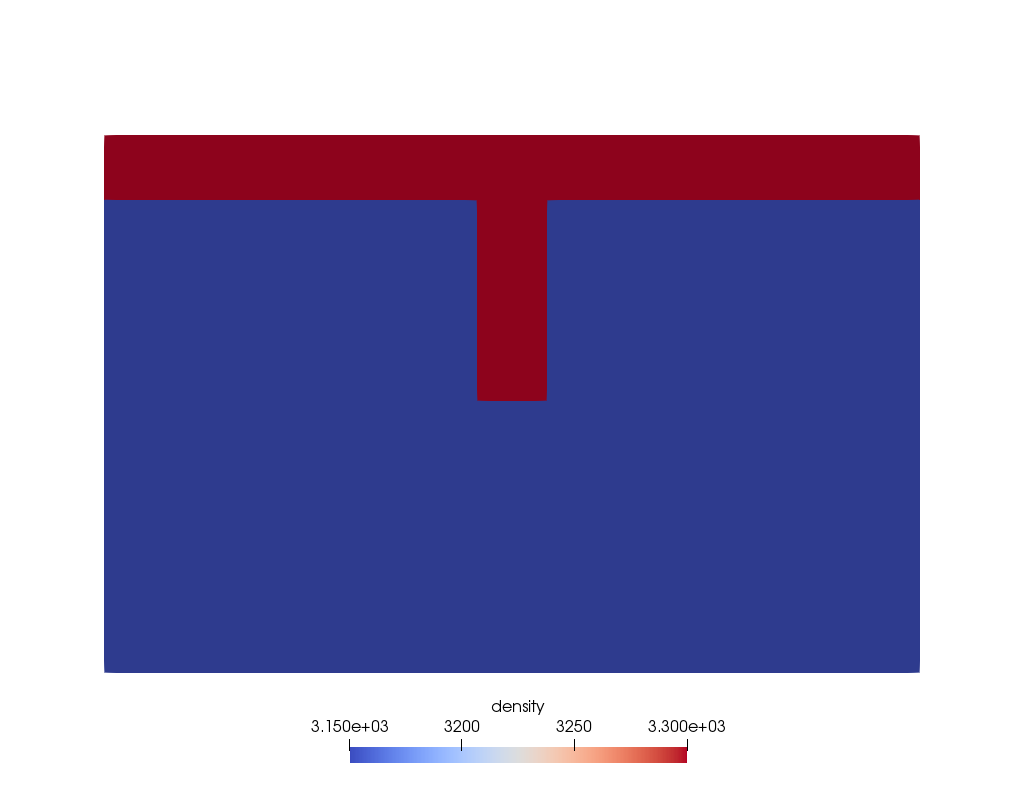
\includegraphics[width=5.cm]{python_codes/fieldstone_slab_detachment1/images/151/density}
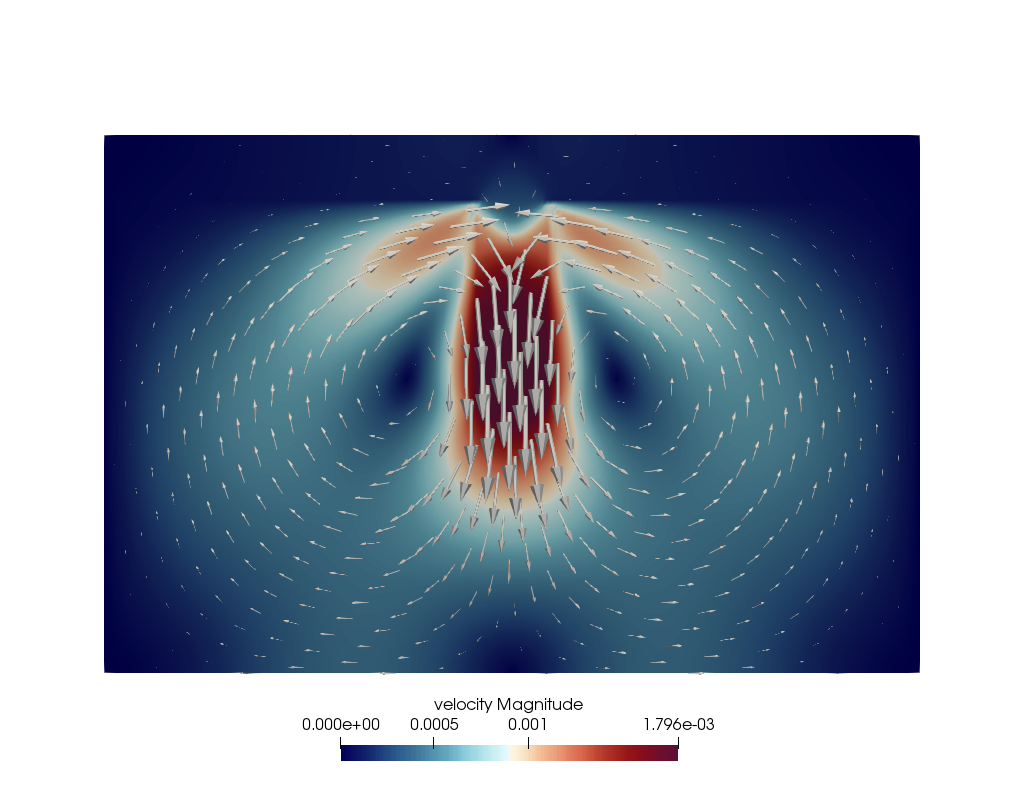
\includegraphics[width=5.cm]{python_codes/fieldstone_slab_detachment1/images/151/velocity}
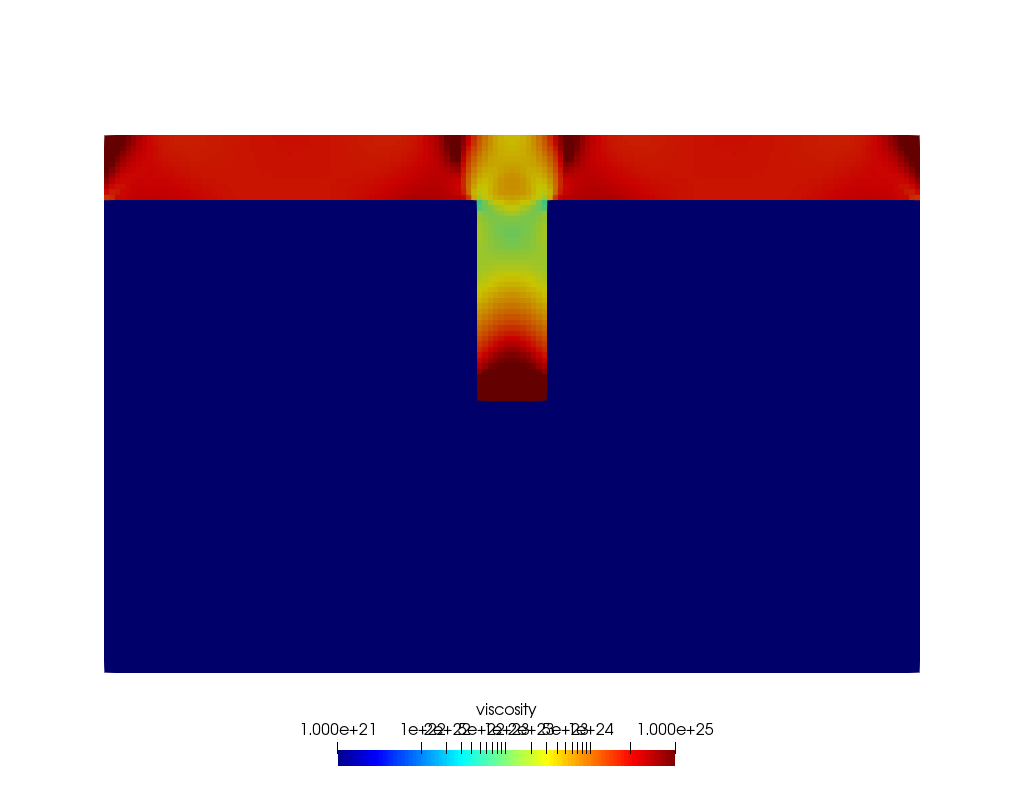
\includegraphics[width=5.cm]{python_codes/fieldstone_slab_detachment1/images/151/viscosity}\\
Fields at convergence for 151x99 grid.
\end{center}




\begin{center}
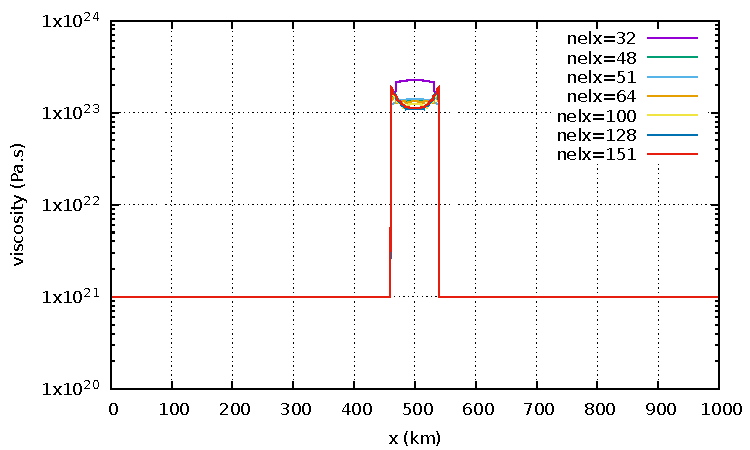
\includegraphics[width=7cm]{python_codes/fieldstone_slab_detachment1/images/horizontal.pdf}
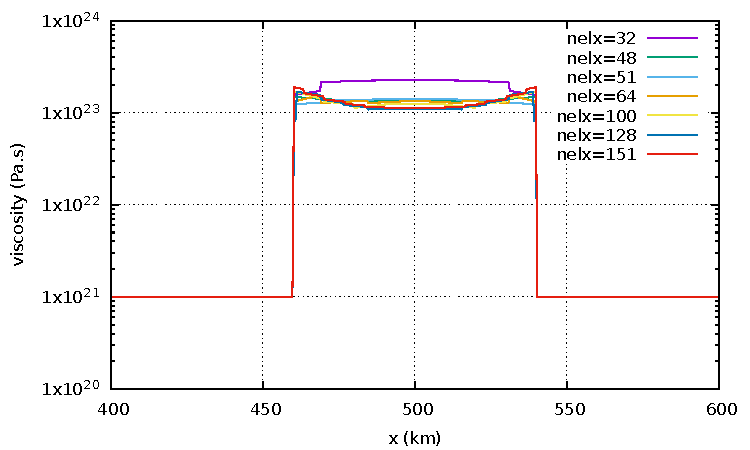
\includegraphics[width=7cm]{python_codes/fieldstone_slab_detachment1/images/horizontal_zoom.pdf}\\
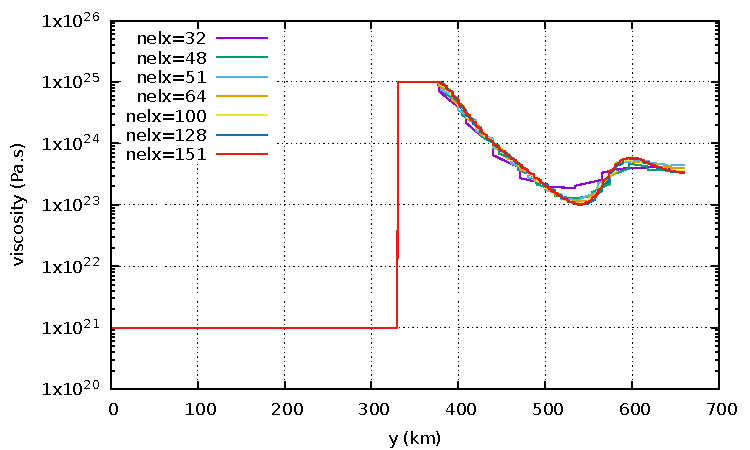
\includegraphics[width=7cm]{python_codes/fieldstone_slab_detachment1/images/vertical.pdf}
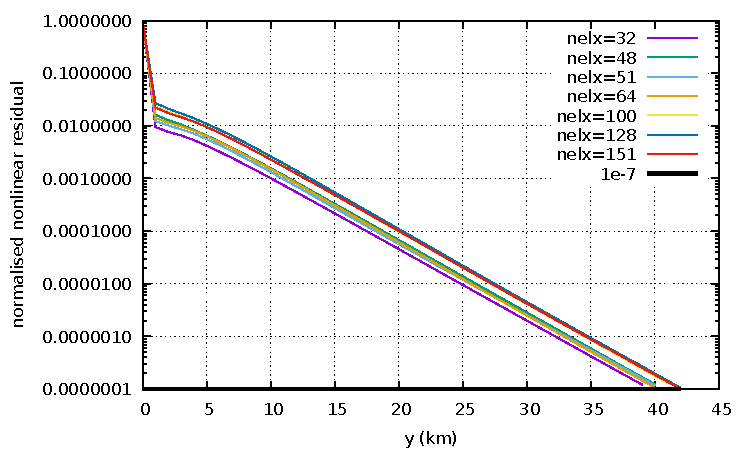
\includegraphics[width=7cm]{python_codes/fieldstone_slab_detachment1/images/residual.pdf}
\end{center}

\begin{center}
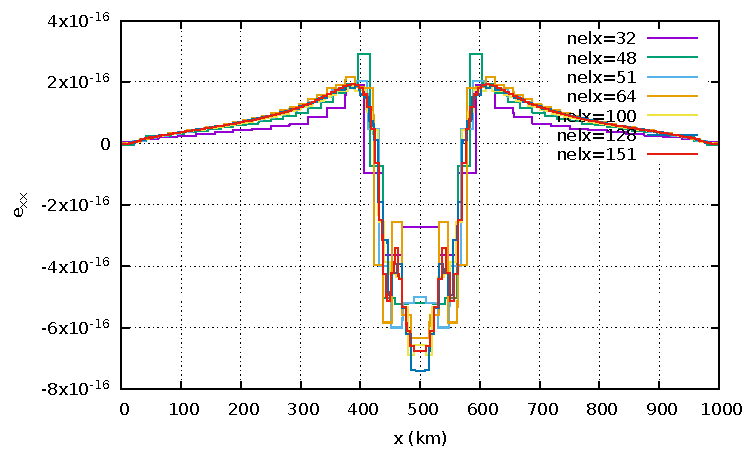
\includegraphics[width=5cm]{python_codes/fieldstone_slab_detachment1/images/horizontal_exx.pdf}
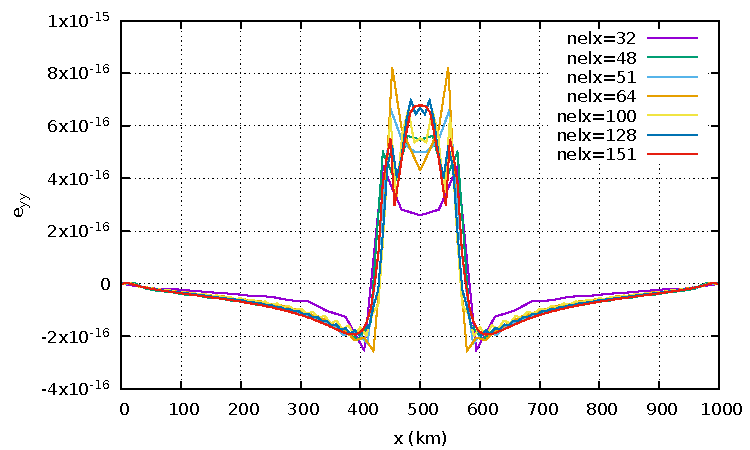
\includegraphics[width=5cm]{python_codes/fieldstone_slab_detachment1/images/horizontal_eyy.pdf}
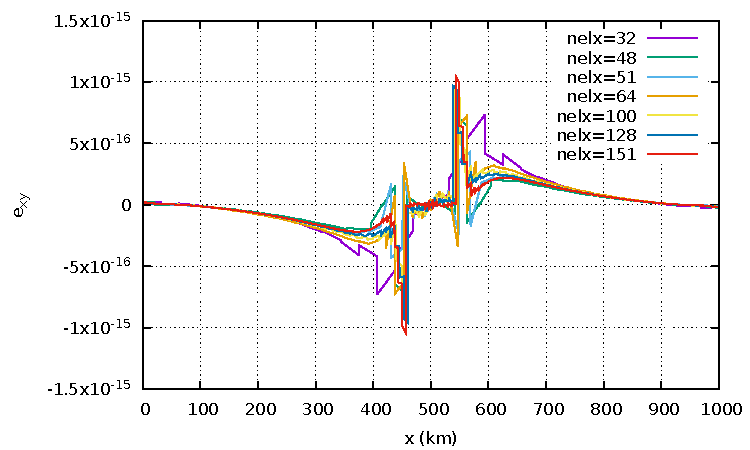
\includegraphics[width=5cm]{python_codes/fieldstone_slab_detachment1/images/horizontal_exy.pdf}\\
Along the horizontal line
\end{center}

\begin{center}
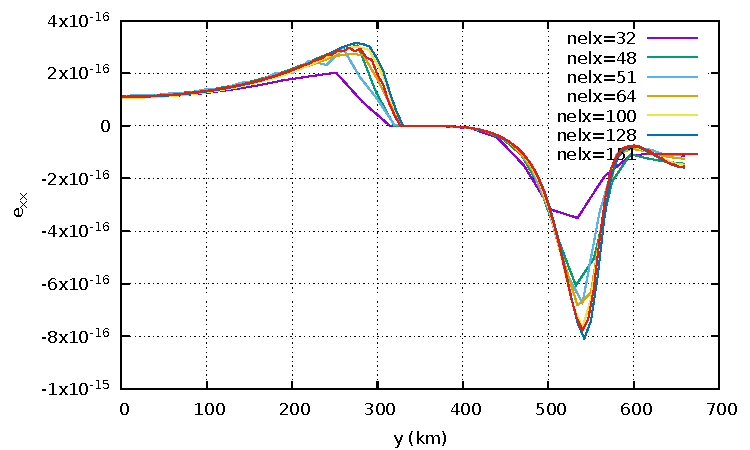
\includegraphics[width=5cm]{python_codes/fieldstone_slab_detachment1/images/vertical_exx.pdf}
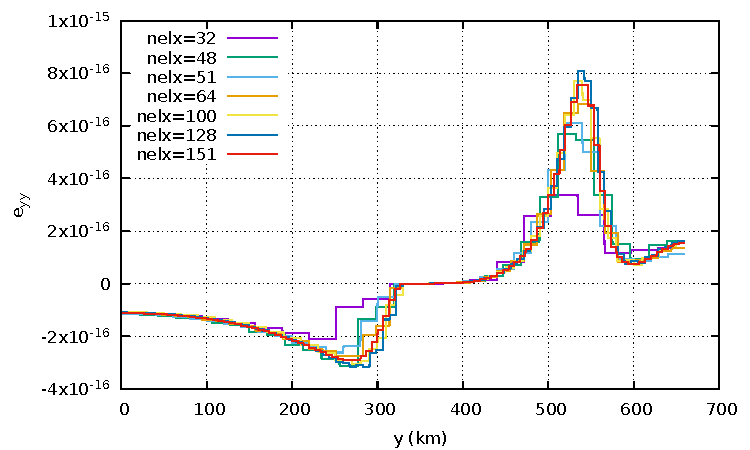
\includegraphics[width=5cm]{python_codes/fieldstone_slab_detachment1/images/vertical_eyy.pdf}
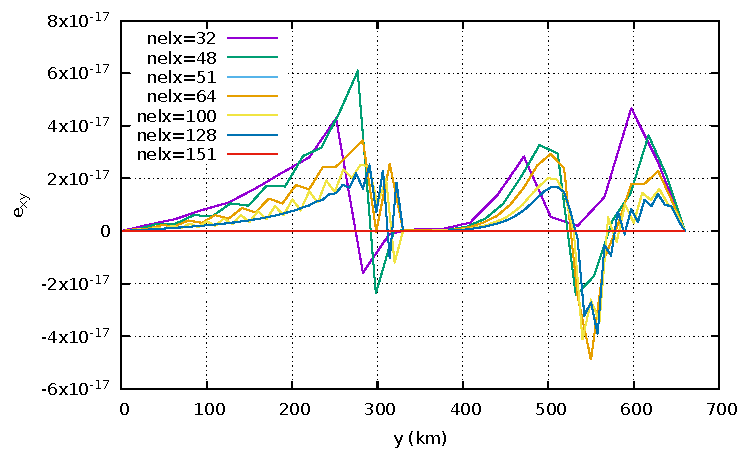
\includegraphics[width=5cm]{python_codes/fieldstone_slab_detachment1/images/vertical_exy.pdf}\\
Along the vertical line
\end{center}



\fbox{
\parbox{10cm}{{\bf features}
\begin{itemize}
\item $Q_1\times P_0$ element \index{$Q_1 \times P_0$}
\item incompressible flow \index{incompressible flow}
\item mixed formulation \index{mixed formulation}
\item isothermal \index{isothermal}
\item nonlinear rheology \index{nonlinear}
\item nonlinear residual
\end{itemize}
}}

Todo: nonlinear mantle, pressure normalisation 

